% ===========================================================================
%
%		FEDERICO II THESIS TEMPLATE - ENGLISH
%  					* an example of Chapter 3: tables, figures and software code
%	 
% 		AUTHOR:  		Antonio Esposito (antonio.esposito103@studenti.unina.it)
%		LAST UPDATED:	2017/06/20
%
% ===========================================================================

\chapter{Testing}

Il documento di testing è mirato a verificare e validare il sistema in modo che sia conforme alle specifiche ed ai requisiti evidenziati dai precedenti documenti.

%%%%% ===============================================================================
\section{Test Plan per il System Testing}
\subsection{Applicativo Desktop}

%Intestazione tabella%
\setcounter{table}{0}
\begin{table}[H]
    \centering
    \footnotesize
    \caption{Test Case \#1}
    \begin{tabularx}{\textwidth}{|c|X|}
        \hline
        Applicativo & Desktop\\
        \hline
        Nome & Amministratore effettua login  \\
        \hline
        Descrizione & Test che assicura il corretto funzionamento del login dell'amministratore\\
        \hline
        Note & Esiste un amministratore con le seguenti credenziali: "admin", "admin" \\
        \hline
        Stato & Passato/Fallito\\
        \hline

    \end{tabularx}
    Continua alla pagina seguente
    \setlength{\tabcolsep}{8pt}
    \renewcommand{\arraystretch}{1.5}
\end{table}
\begin{table}[H]
    \footnotesize
    \begin{tabularx}{\textwidth}{|c|X|X|X|}
        \hline
        Step\# & Input & Risultato Atteso & Risultato Ottenuto \\
        \hline
         1 & Viene aperto l'applicativo Desktop  
         & Viene visualizzata la schermata "Login" contententue due Textbox (Username e Password) 
         ed un tasto
         &DA INSERIRE (Come ci si aspettava)\\
          \hline
        2 & Vengono inserite delle credenziali \textbf{errate} "0000", "0000" e viene cliccato 
        il tasto "Login" 
        & Il login fallisce e viene visualizzata il dialog "Credenziali errate"
        & DA INSERIRE\\
         \hline
         3 & Viene premuto il tasto "OK"
        & Viene mostrata nuovamente la schermata di login
        & DA INSERIRE\\
        4 & Vengono inserite le credenziali "admin", "admin" e viene cliccato 
        il tasto "Login" 
        & Il login ha successo e viene visualizzata la schermata "
        Revisioni" 
        & DA INSERIRE\\
         \hline
                 
    \end{tabularx}
\end{table}
    
       


%Intestazione tabella%
\begin{table}[H]
    \footnotesize
    \caption{Test Case \#2}
    \begin{tabularx}{\textwidth}{|c|X|}
        \hline
        Applicativo & Desktop\\
        \hline
        Nome & Amministratore visualizza dati di un utente  \\
        \hline
        Descrizione & Test che assicura il corretto funzionamento della visualizzazione dei dati dell'utente\\
        \hline
        Note & L'amministratore deve essere loggato, deve esistere l'utente con nickname "utente" \\
        \hline
        Stato & Passato/Fallito\\
        \hline

    \end{tabularx}
    \setlength{\tabcolsep}{8pt}
    \renewcommand{\arraystretch}{1.5}
\end{table}

\begin{table}[H]
    \footnotesize
    \begin{tabularx}{\textwidth}{|c|X|X|X|}
        \hline
        Step\# & Input & Risultato Atteso & Risultato Ottenuto \\
        \hline
         1 & Viene premuto il tasto "Visitatori" dalla schermata "Recensioni" 
         & Viene visualizzata la schermata "Visitatori" contententue una lista di visitatori
         &Come ci si aspettava \\
          \hline
        2 & Viene cliccata la riga contenente l'utente con nickname "utente"
        & Viene visualizzata la schermata utente contenete i tasti "Modifica", "Elimina" ed i textfild nome, nickname, data di nascita, email, recensioni rifiutate ed approvate contenenti i relativi dati.
        & Come ci si aspettava\\
         \hline  
    \end{tabularx}
\end{table}
    
       

\pagebreak
%Intestazione tabella%
\begin{table}[H]
    \centering
    \footnotesize
    \caption{Test Case \#3}
    \begin{tabularx}{\textwidth}{|c|X|}
        \hline
        Applicativo & Desktop\\
        \hline
        Nome & Amministratore valuta una recensione  \\
        \hline
        Descrizione & Test che assicura il corretto funzionamento della valutazione delle recensioni\\
        \hline
        Note & L'amministatore deve essere autenticato e deve esistere una recensione scritta da "utente" per la struttura "Struttura" in data "GEN 1 2020" \\
        \hline
        Stato & Passato/Fallito\\
        \hline

    \end{tabularx}
    Continua alla pagina seguente
    \setlength{\tabcolsep}{8pt}
    \renewcommand{\arraystretch}{1.5}
\end{table}

\begin{table}[H]
    \footnotesize
    \begin{tabularx}{\textwidth}{|c|X|X|X|}
        \hline
        Step\# & Input & Risultato Atteso & Risultato Ottenuto \\
        \hline
         1 & Viene premuto il tasto "Recensioni" dalla schermata "Visitatori" 
         & Viene visualizzata la schermata "Recensioni" contententue una lista di recensioni
         &DA INSERIRE (Come ci si aspettava)\\
          \hline
        2 & Viene cliccata la riga contenente la recensione scritta in data "GEN 1 2020" dall'utente "utente" sulla struttura "Struttura"
        & Viene visualizzata la schermata della recensione contenete i tasti "Acceta" e  "Rifiuta", i textFiel contenenti il titolo, il testo e l'autore della descrizione.
        Viene visualizzato, in oltre, il numero di stelline della recensione.
        & DA INSERIRE\\
         \hline 
        3 & Viene cliccato il bottone "Accetta" o "Rifiuta"
         & Viene visualizzato il dialog che ci informa che l'azione è stata svolta con successo
         & DA INSERIRE\\
          \hline
          4 & Viene premuto il tasto "Ok"
         & Viene visualizzata la schermata Recensioni e nella lista delle recensioni non compare più 
         la recensione scritta dall'utente "Utente" sulla struttura "Struttura" in data "GEN 1 2020"
         & DA INSERIRE\\
          \hline      
    \end{tabularx}
\end{table}
    
       


%Intestazione tabella%
\begin{table}[H]
    \centering
    \footnotesize
    \caption{Test Case \#4}
    \begin{tabularx}{\textwidth}{|c|X|}
        \hline
        Applicativo & Desktop\\
        \hline
        Nome & Amministratore elimina visitatore  \\
        \hline
        Descrizione & Test che assicura il corretto funzionamento dell'eliminazione di un visitatore'\\
        \hline
        Note & L'amministatore deve essere autenticato e deve esistere l'utente "utente"  \\
        \hline
        Stato & Passato/Fallito\\
        \hline

    \end{tabularx}
    Continua alla pagina seguente
    \setlength{\tabcolsep}{8pt}
    \renewcommand{\arraystretch}{1.5}
\end{table}
%Step%
\begin{table}[H]
    \footnotesize
    \begin{tabularx}{\textwidth}{|c|X|X|X|}
        \hline
        Step\# & Input & Risultato Atteso & Risultato Ottenuto \\
        \hline
         1 & Viene premuto il tasto "Visitatori" dalla schermata "Recensioni" 
         & Viene visualizzata la schermata "Visitatori" contententue una lista di visitatori
         &Come ci si aspettava\\
          \hline
        2 & Viene cliccata la riga contenente l'utente "utente"
        & Viene visualizzata la schermata di visualizzazione dell'utente contenente i bottoni "Elimina" e "Modifica"
          Sulla schermata sono presenti anche i seguenti textfield: nome, email, nickname, data di nascita, recensioni approvate e rifiutate .
        & Come ci si aspettava\\
         \hline 
        3 & Viene cliccato il bottone "Elimina"
         & Viene visualizzato il dialog che ci informa che l'utente è stato eliminato con successo
         & Come ci si aspettava\\
          \hline
          4 & Viene premuto il tasto "Ok"
         & Viene visualizzata visualizzata nuovamente la schermata con la lista dei visitatori
         & Come ci si aspettava\\
          \hline      
    \end{tabularx}
\end{table}
    
       


%Intestazione tabella%
\begin{table}[H]
    \centering
    \footnotesize
    \caption{Test Case \#5}
    \begin{tabularx}{\textwidth}{|c|X|}
        \hline
        Applicativo & Desktop\\
        \hline
        Nome & Amministratore modifica dati visitatore  \\
        \hline
        Descrizione & Test che assicura il corretto funzionamento della modifica dei dati di un visitatore'\\
        \hline
        Note & L'amministatore deve essere autenticato e deve esistere l'utente "utente" con nickname "user"  \\
        \hline
        Stato & Passato/Fallito\\
        \hline

    \end{tabularx}
    Continua alla pagina seguente
    \setlength{\tabcolsep}{8pt}
    \renewcommand{\arraystretch}{1.5}
\end{table}
%Step%
\begin{table}[H]
    \footnotesize
    \begin{tabularx}{\textwidth}{|c|X|X|X|}
        \hline
        Step\# & Input & Risultato Atteso & Risultato Ottenuto \\
        \hline
         1 & Viene premuto il tasto "Visitatori" dalla schermata "Recensioni" 
         & Viene visualizzata la schermata "Visitatori" contententue una lista di visitatori
         &DA INSERIRE (Come ci si aspettava)\\
          \hline
        2 & Viene cliccata la riga contenente l'utente "utente"
        & Viene visualizzata la schermata di visualizzazione dell'utente contenente i bottoni "Elimina" e "Modifica"
          Sulla schermata sono presenti anche i seguenti textfield: nome, email, nickname, data di nascita, recensioni approvate e rifiutate .
        & DA INSERIRE\\
         \hline 
        3 & Viene cliccato il bottone "Modifica"
         & Viene visualizzata la schemata di modifica dei tasti utente contenente due editText ("Nickname" e "Password") e
         due bottoni ("Annulla" e "Conferma")
         & DA INSERIRE\\
          \hline
        4 & Viene inserito il Nickname "user" e la nuova password: "pass"; viene premuto il tasto "Ok"
         & Viene visualizzata un dialog che avvisa che l'azione non ha avuto successo
         & DA INSERIRE\\
          \hline  
          5 & Viene premuto il tasto "OK"
          & Viene visualizzata nuovamente la schermata contenente le informazioni di "utente"
          & DA INSERIRE\\
          \hline      
        6 & Viene inserito il Nickname "nuovoNickname" e la nuova password: "pass"; viene premuto il tasto "Ok"
         & Viene visualizzata un dialog che avvisa che l'azione ha avuto successo
         & DA INSERIRE\\
           \hline 
           7 & Viene premuto il tasto "Ok"
           & Viene visualizzata nuovamente la schermata con le informazioni dell'utente e
           viene visualizzato il nickname ("nuovoNickname")
           & DA INSERIRE\\
             \hline                       
    \end{tabularx}
\end{table}
    
       


\pagebreak
\subsection{Applicativo Mobile}

%Intestazione tabella%
\begin{table}[H]
    \centering
    \footnotesize
    \caption{Test Case \#1}
    \begin{tabularx}{\textwidth}{|c|X|}
        \hline
        Applicativo & Mobile\\
        \hline
        Nome & Utente si registra alla piattaforma  \\
        \hline
        Descrizione & Test che assicura il corretto funzionamento della funzione di registrazione\\
        \hline
        Note &  L'utente non deve aver effettuato il login e non deve esistere nessun utente
         registrato con i seguenti dati: nickname = "nick" email = "email.email@gmail.com".\\
        \hline
        Stato & Passato/Fallito\\
        \hline

    \end{tabularx}
    %Continua alla pagina seguente
    \setlength{\tabcolsep}{8pt}
    \renewcommand{\arraystretch}{1.5}
\end{table}
%Step%
\begin{table}[H]
    \footnotesize
    \begin{tabularx}{\textwidth}{|c|X|X|X|}
        \hline
        Step\# & Input & Risultato Atteso & Risultato Ottenuto \\
        \hline
         1 & Dall'homepage viene cliccata l'iconda del menù in alto a sinistra 
         & Viene visualizzato il menù laterale sinsitra
         &Come ci si aspettava \\
          \hline
        2 & Viene cliccata la riga contenente "Registrati"
        & Viene visualizzata la schermata di registrazione con il bottone "Fine", 5 TextField, 1 datePicker ed una checkbox
        & Come ci si aspettava\\
         \hline 
        3 & Non viene compilato nessun campo e viene premuto il tasto "Fine"
         & Viene mostrato un dialog di errore & Come ci si aspettava\\
          \hline
        4 & Viene premuto il tasto "Ok"
         & Viene visualizzata nuovamente la schermata di registrazione
         & Come ci si aspettava\\
          \hline 
          5 & Vengono inseriti i campi: "email.email@gmail.com", "password","Mario",
          "Rossi", "17/11/1998", "nick" e viene premuto il tasto "Fine".
         & Viene visualizzata mostrato il dialog di registrazione effettuata
         & Come ci si aspettava\\
          \hline           
    \end{tabularx}
\end{table}
    
       


%Intestazione tabella%
\begin{table}[H]
    \centering
    \footnotesize
    \caption{Test Case \#2}
    \begin{tabularx}{\textwidth}{|c|X|}
        \hline
        Applicativo & Mobile\\
        \hline
        Nome & Utente accede alla piattaforma  \\
        \hline
        Descrizione & Test che assicura il corretto funzionamento della funzione di Login\\
        \hline
        Note &  L'utente non deve aver effettuato il login e deve esistere l'utente
        con nickname="nickname" e password "password"\\
        \hline
        Stato & Passato/Fallito\\
        \hline

    \end{tabularx}
    Continua alla pagina seguente
    \setlength{\tabcolsep}{8pt}
    \renewcommand{\arraystretch}{1.5}
\end{table}
%Step%
\begin{table}[H]
    \footnotesize
    \begin{tabularx}{\textwidth}{|c|X|X|X|}
        \hline
        Step\# & Input & Risultato Atteso & Risultato Ottenuto \\
        \hline
         1 & Dall'homepage viene cliccata l'iconda del menù in alto a sinistra 
         & Viene visualizzato il menù laterale sinsitra
         &Come ci si aspettava \\
          \hline
        2 & Viene cliccata la riga contenente "Login"
        & Viene visualizzata la schermata di Login con il bottone "Login" 2 TextField
        & Come ci si aspettava\\
         \hline 
        3 & Non viene compilato nessun campo e viene premuto il tasto "Fine"
         & Viene mostrato un dialog di errore & Come ci si aspettava\\
          \hline
        4 & Viene premuto il tasto "Ok"
         & Viene visualizzata nuovamente la schermata di Login
         & Come ci si aspettava\\
          \hline 
          5 & Vengono inseriti i campi: "nickname" e "password" e viene premuto il tasto "Login"
         & Viene visualizzata mostrata la homepage dell'applicativo
         & Come ci si aspettava\\
          \hline           
    \end{tabularx}
\end{table}
    
       


%Intestazione tabella%
\begin{table}[H]
    \centering
    \footnotesize
    \caption{Test Case \#3}
    \begin{tabularx}{\textwidth}{|c|X|}
        \hline
        Applicativo & Mobile\\
        \hline
        Nome & Utente aggiunge una recensione  \\
        \hline
        Descrizione & Test che assicura il corretto funzionamento dell'aggiunta di recensioni\\
        \hline
        Note &  L'utente deve aver effettuato il login\\
        \hline
        Stato & Passato/Fallito\\
        \hline

    \end{tabularx}
    Continua alla pagina seguente
    \setlength{\tabcolsep}{8pt}
    \renewcommand{\arraystretch}{1.5}
\end{table}
%Step%
\begin{table}[H]
    \footnotesize
    \begin{tabularx}{\textwidth}{|c|X|X|X|}
        \hline
        Step\# & Input & Risultato Atteso & Risultato Ottenuto \\
        \hline
         1 & Viene aperta la schermata di visualizzazione di una struttura
         & Viene visualizzato una schermata contenente tutti i dettagli della struttura
         &DA INSERIRE (Come ci si aspettava)\\
          \hline
        2 & Viene cliccato il pulsante "Aggiungi Recensione"
        & Viene visualizzata la schermata di aggiunta recensione
        & DA INSERIRE\\
         \hline 
        3 & Non viene compilato nessun campo e viene premuto il tasto "Fine"
         & Viene mostrato un dialog di errore & DA INSERIRE\\
          \hline
        4 & Viene premuto il tasto "Ok"
         & Viene visualizzata nuovamente la schermata di Login
         & DA INSERIRE\\
          \hline 
          5 & Vengono inseriti i campi: "titolo", "testo", viene cliccata la prima stellina a sinistra e viene premuto il tasto "Aggiungi"
         & Viene visualizzato dialog che notifica l'avvenuta operazione.
         & DA INSERIRE\\
          \hline 
          6 & Preme "Ok"
          & Viene visualizzato nuovamente la schermata della struttura
          & DA INSERIRE\\
           \hline                     
    \end{tabularx}
\end{table}
    
       


%Intestazione tabella%
\begin{table}[H]
    \centering
    \footnotesize
    \caption{Test Case \#4}
    \begin{tabularx}{\textwidth}{|c|X|}
        \hline
        Applicativo & Mobile\\
        \hline
        Nome & Utente visualizza una struttura  \\
        \hline
        Descrizione & Test che assicura il corretto funzionamento della visualizzazione di una struttra\\
        \hline
        Note &  Deve esistere la struttura "Struttura"\\
        \hline
        Stato & Passato/Fallito\\
        \hline

    \end{tabularx}
   %Continua alla pagina seguente
    \setlength{\tabcolsep}{8pt}
    \renewcommand{\arraystretch}{1.5}
\end{table}
%Step%
\begin{table}[H]
    \footnotesize
    \begin{tabularx}{\textwidth}{|c|X|X|X|}
        \hline
        Step\# & Input & Risultato Atteso & Risultato Ottenuto \\
        \hline
         1 & Viene aperta la lista di strutture in seguito ad una ricerca inserendo "Struttura" come nome
         & Viene visualizzato una schermata contenente tutte le strutture che rispettano i criteri di ricerca
         &DA INSERIRE (Come ci si aspettava)\\
          \hline
        2 & Viene cliccata la card della struttura "Struttura"
        & Viene visualizzata la schermata contenente tutti i dettagli della struttura
        & DA INSERIRE\\
         \hline 
        
    \end{tabularx}
\end{table}
    
       


%Intestazione tabella%
\begin{table}[H]
    \centering
    \footnotesize
    \caption{Test Case \#5}
    \begin{tabularx}{\textwidth}{|c|X|}
        \hline
        Applicativo & Mobile\\
        \hline
        Nome & Utente visualizza i dettagli di una struttura  \\
        \hline
        Descrizione & Test che assicura il corretto funzionamento della visualizzazione di una struttura\\
        \hline
        Note & Esiste la struttura "struttura"\\
        \hline
        Stato & Passato/Fallito\\
        \hline

    \end{tabularx}
    %Continua alla pagina seguente
    \setlength{\tabcolsep}{8pt}
    \renewcommand{\arraystretch}{1.5}
\end{table}
%Step%

\begin{table}[H]
    \footnotesize
    \begin{tabularx}{\textwidth}{|c|X|X|X|}
        \hline
        Step\# & Input & Risultato Atteso & Risultato Ottenuto \\
        \hline
         1 & Viene ricercata la struttura "Struttura"
         & Viene visualizzato una lista di strutture con il nome "Struttura"
         &DA INSERIRE (Come ci si aspettava)\\
          \hline
        2 & Viene cliccata sulla card della prima struttura
        & Viene visualizzata la schermata della struttura
        & DA INSERIRE\\
\hline
    \end{tabularx}
\end{table}
    
       


%Intestazione tabella%
\begin{table}[H]
    \centering
    \footnotesize
    \caption{Test Case \#6}
    \begin{tabularx}{\textwidth}{|c|X|}
        \hline
        Applicativo & Mobile\\
        \hline
        Nome & Utente visualizza i dettagli di una recensione  \\
        \hline
        Descrizione & Test che assicura il corretto funzionamento della visualizzazione di una recensione\\
        \hline
        Note & Esiste una recensione alla struttura "struttura"\\
        \hline
        Stato & Passato/Fallito\\
        \hline

    \end{tabularx}
    %Continua alla pagina seguente
    \setlength{\tabcolsep}{8pt}
    \renewcommand{\arraystretch}{1.5}
\end{table}
%Step%

\begin{table}[H]
    \footnotesize
    \begin{tabularx}{\textwidth}{|c|X|X|X|}
        \hline
        Step\# & Input & Risultato Atteso & Risultato Ottenuto \\
        \hline
         1 & Viene aperta la pagina struttura "Struttura"
         & Vengono visualizzati i dati della struttura ed una lista di recensioni
         &DA INSERIRE (Come ci si aspettava)\\
          \hline
        2 & Viene cliccata sulla card della prima recensione
        & Viene visualizzata la schermata contenente i dettagli della recensione
        & DA INSERIRE\\
\hline
    \end{tabularx}
\end{table}
    
       


%Intestazione tabella%
\begin{table}[H]
    \centering
    \footnotesize
    \caption{Test Case \#7}
    \begin{tabularx}{\textwidth}{|c|X|}
        \hline
        Applicativo & Mobile\\
        \hline
        Nome & Utente visualizza una struttura su mappa  \\
        \hline
        Descrizione & Test che assicura il corretto funzionamento della visualizzazione su mappa di una struttura\\
        \hline
        Note & \\
        \hline
        Stato & Passato/Fallito\\
        \hline

    \end{tabularx}
    %Continua alla pagina seguente
    \setlength{\tabcolsep}{8pt}
    \renewcommand{\arraystretch}{1.5}
\end{table}
%Step%

\begin{table}[H]
    \footnotesize
    \begin{tabularx}{\textwidth}{|c|X|X|X|}
        \hline
        Step\# & Input & Risultato Atteso & Risultato Ottenuto \\
        \hline
         1 & Viene aperta la pagina struttura "Struttura"
         & Vengono visualizzati i dati della struttura ed una lista di recensioni
         &Come ci si aspettava \\
          \hline
        2 & Viene cliccato sul bottone in basso a destra
        & Viene visualizzata l'icona della visualizzazione su mappa
        & Come ci si aspettava\\
        3 & Viene cliccata l'icona della visualizzazione su mappa
        & Viene aperta la schemata di visualizzazione su mappa che mostra la posizione della struttura sulla mappa.
        & Come ci si aspettava\\
\hline
    \end{tabularx}
\end{table}
    
       

\pagebreak
\section{Codice jUnit per unit testing}
\subsection{Testing Black Box}
Effettueremo una serie di test, tramite strategia Strong Equivalence Class Testing sul seguente metodo:
\begin{lstlisting}
public boolean tryLogin(String username, String password)
\end{lstlisting}
Definiamo le classi di equivalenza dei valori assumibili dai parametri in input:
%Intestazione tabella%
\begin{table}[H]
    \centering
    \footnotesize
    \caption{Classi di equivalenza di 'username'}
    \begin{tabularx}{\textwidth}{|c|X|}
        \hline
        Classe di Equivalenza & Descrizione\\
        \hline
        EC1 & username è null  \\
        \hline
        EC2 & username è una stringa vuota\\
        \hline
        EC3 &  username è sbagliato\\
        \hline
        EC4 & username è corretto\\
        \hline
    \end{tabularx}
    %Continua alla pagina seguente
    \setlength{\tabcolsep}{8pt}
    \renewcommand{\arraystretch}{1.5}
\end{table}
\begin{table}[H]
    \centering
    \footnotesize
    \caption{Classi di equivalenza di 'password'}
    \begin{tabularx}{\textwidth}{|c|X|}
        \hline
        Classe di Equivalenza & Descrizione\\
        \hline
        EC5 & password è null  \\
        \hline
        EC6 & password è una stringa vuota\\
        \hline
        EC7 &  password è sbagliata\\
        \hline
        EC8 & password è corretta\\
        \hline
    \end{tabularx}
    %Continua alla pagina seguente
    \setlength{\tabcolsep}{8pt}
    \renewcommand{\arraystretch}{1.5}
\end{table}
Effettuiamo il prodotto cartesiano tra le classi di equivalenza del primo parametro 
e quelle del secondo parametro per ottenere tutti i possibili testcase.

\begin{table}[H]
    \centering
    \footnotesize
    \caption{Lista dei TestCase}
    \begin{tabularx}{\textwidth}{|c|X|X|}
        \hline
        Test Case & Classe di Equivalenza & Descrizione\\
        \hline
        TC1 & EC1 & EC5  \\
        \hline
        TC2 & EC1 & EC6  \\
        \hline
        TC3 & EC1 & EC7  \\
        \hline
        TC4 & EC1 & EC8  \\
        \hline
        TC5 & EC2 & EC5  \\
        \hline
        TC6 & EC2 & EC6  \\
        \hline
        TC7 & EC2 & EC7  \\
        \hline
        TC8 & EC2 & EC8  \\
        \hline
        TC9 & EC3 & EC5  \\
        \hline
        TC10 & EC3 & EC6  \\
        \hline
        TC11 & EC3 & EC7  \\
        \hline
        TC12 & EC3 & EC8  \\
        \hline
        TC13 & EC4 & EC5  \\
        \hline
        TC14 & EC4 & EC6  \\
        \hline
        TC15 & EC4 & EC7  \\
        \hline
        TC16 & EC4 & EC8  \\
        \hline
    \end{tabularx}
    %Continua alla pagina seguente
    \setlength{\tabcolsep}{8pt}
    \renewcommand{\arraystretch}{1.5}
\end{table}
\begin{table}[H]
    \centering
    \footnotesize
    \caption{Precondizioni}
    \begin{tabularx}{\textwidth}{|c|c|X|}
        \hline
        Precondizione & Input & Output Atteso\\
        \hline
        'admin' ha diritto d'accesso & "admin", "admin" & true\\
        \hline
        'sbagliato' non ha diritto d'accesso & "sbagliato" , "sbagliato" & false\\
        \hline
    \end{tabularx}
\end{table}

\lstinputlisting[caption=Casi di test]{TestCases/AdminDAO_TestSuite.java}


       

\pagebreak
\subsection{Testing Whitebox}
\begin{center}
    \begin{figure}[h]
        \centering
        \caption{Grafo di copertura della funzione}
        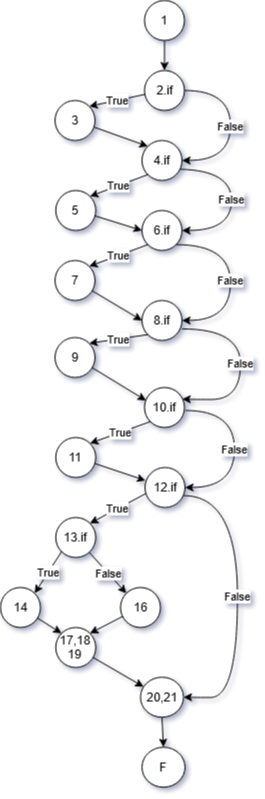
\includegraphics[scale=0.5]{Figures/Grafo di copertura.png}
    \end{figure}
\end{center}